\chapter{Background}
\label{cha:background}
To fully understand the extent of this project it is important to understand how Wikipedia works. In this chapter I will provide an introduction to Wikipedia, its community and some relevant internal dynamics. I will also introduce some of the dataset and libraries we used.


\section{Wikipedia}
\label{sec:wikipedia}
Wikipedia is a free, multilingual online encyclopedia written and maintained by a community of volunteer contributors through a model of open collaboration. Wikipedia contents are divided into pages, and pages are written by editors.


There exist 323 language editions of Wikipedia. Each edition has different pages and slightly different rules. The most popular edition is the English one, which receives 48\% of Wikipedia cumulative traffic.


The total number of pages in all languages is 233 million; 57 millions of these are articles and 6 million of those are in English. English articles, not only are the most common but are also considered the most accurate, solid, and exhaustive. It is a good approximation to say that 2/3 of Wikipedia is written in English.


Wikipedia pages are grouped into namespaces, which separates data into core sets, differentiating content for public viewing and content intended for the editing community. The more relevant namespaces are “Articles” that contains the actual encyclopedia; “Talk”, where editor discuss improvement to articles; “User”, that contains interpersonal discussion and personal content; “User Talk”, where user can send messages to each other.


All Wikipedia pages are written in \textit{Wikitext}, a special markup language used to graphically represent a page structure. All content is backed up and saved in a dump file every month and made publicly available. The dump contains all modifications made to every Wikipedia page at all times.



\subsection{Wikipedia Users}
\label{sec:wikipediausers}
Wikipedia pages can be edited by registered or anonymously users. As of June 2021, there are 96 million accounts, of which about 310 thousand have made at least one edit in the last thirty days and are considered active.


Wikipedia users have different abilities to perform specific actions based on the user groups they are in. The most popular user groups and the ones of relevance for this study are:
\begin{itemize}
\item \textbf{Unregistered}: Users who are not logged in and are identified by their IP Address.
\item \textbf{Registered}: Users that are logged in with an email and have obtained a username.
\item \textbf{Autoconfirmed}: User that are at least four days old and have made at least 10 edits.
\item \textbf{Autopatrolled}: Editors whose articles are automatically marked as “reviewed” by the system.
\item \textbf{Administrators (or sysop)}: Editors who are granted by the community exclusive access to several tools, to allow them to carry out certain functions.
\item \textbf{Bots}: Virtual users that run automated tasks on pages. Usually, they are programmed by other users to perform simple and repetitive tasks, much faster than a person could.
\end{itemize}

Users have a “User page” where they can give basic information about themselves and their work on the platform and related projects. Users can also specify some information about themselves on the preference page, such as their username, their signature, or their gender.


A feature of relevant importance in this research is UserBoxes.\footnote{\url{https://en.wikipedia.org/wiki/Wikipedia:Userboxes}} They are graphical decoration users can add to their page and consists of a colored rectangle with some text and, sometimes, a picture, used to provide a notice about a user. UserBoxes are often embedded into a user page through a pre-made template, making them similar between multiple users. 


\subsection{Wikipedia talk pages}
\label{sec:wikipediatalkpages}
Talk pages can be of two kinds: “Article talk pages” and “User talk pages”.

“Article talk pages” is the second biggest namespace in Wikipedia, after “Articles”. Each Wikipedia article has an article talk page, which is an administrative page where editors can discuss improvements to other articles or Wikipedia pages.

Any user page has a corresponding “user talk page” that can be used by other users to send messages or discuss with other users.

The focus of this research is on these pages since users can express their emotions more freely and interact with each other directly. Talk pages are divided into threads, which groups user’s posts on a topic of discussion. Each post is made by a user, and it can start a new thread or reply to an existing one. At the end of a post, a user is highly encouraged to leave his username and the current date. Several guidelines on these pages structure can be followed by editors, to have consistency on all pages.

\begin{figure}[H]
    \centering
    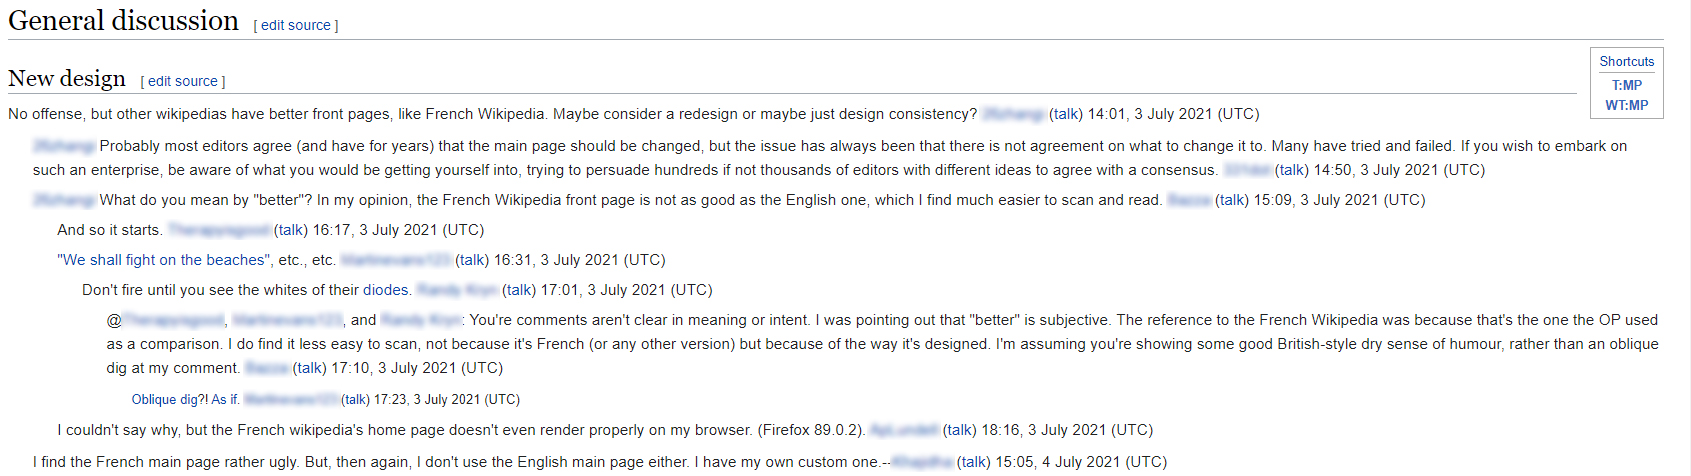
\includegraphics[width=1\textwidth]{./img/discussion.jpg}
    \caption{Example of a discussion on a talk page}
    \label{fig:discussion}
\end{figure}


\section{WikiConv Dataset}
\label{sec:wikiconvdataset}
WikiConv is a multilingual corpus encompassing the history of conversations on Wikipedia Talk Pages, including deletion, modification, and restoration of comments, called actions.\footnote{\url{https://github.com/conversationai/wikidetox/tree/main/wikiconv}} The version we used includes all conversations extracted from the 2020-01-04 Wikipedia dumps of English, Spanish, Italian, and Catalan.

Each language version of the dataset is split into smaller files compressed through gzip. The files contain an action for each line.

\begin{table}[H]
    \centering
    \ra{1.2}
    \begin{tabularx}{\columnwidth}{@{}Xrrrr@{}}
        \midrule
        \textbf{Language} & \textbf{Number of actions} & \textbf{Number of files} & \textbf{Size of files} & \textbf{Total size}\\ \toprule
        English & 235 Millions & 50 & 2.5 GB & 485 GB \\
        Spanish & 20 Millions & 5 & 2 GB & 41 GB \\
        Italian & 17 Millions & 5 & 2 GB & 41 GB \\
        Catalan & 2 Millions & 1 & 2 GB & 7 GB \\

         \bottomrule
    \end{tabularx}
    
    \caption{Size of the WikiConv Dataset in various languages.  \label{table:datasetsize}}
\end{table}

An edit of a page by a user is called revision, and can be represented by several action of four different kinds:

\begin{itemize}
\item \textbf{Creation}: An edit that creates a new section in a Wikipedia page.
\item \textbf{Addition}: An edit that adds a new post to a thread.
\item \textbf{Modification}: An edit that modifies an existing post.
\item \textbf{Deletion}: An edit that removes a post.
\item \textbf{Restoration}: An edit that restores a previously removed post.
\end{itemize}

Each action is a JSON object that contains several pieces of information, as listed on the dataset documentation. The most relevant data for this study is: the page title and page id; the user name and id; the text of the post underlying the action; the timestamp of the revision and the type of action.


\begin{figure}[H]
    \centering
    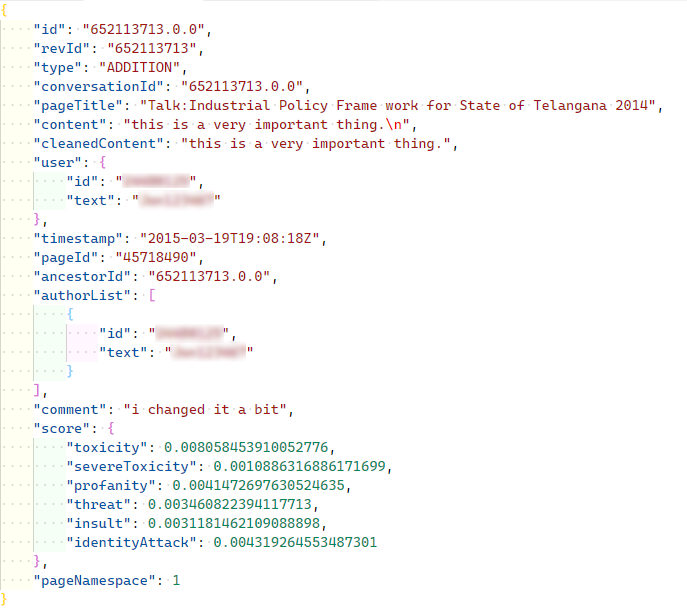
\includegraphics[width=0.7\textwidth]{./img/wikiconv.png}
    \caption{Example of an action contained in the English WikiCovn}
    \label{fig:wikiconv}
\end{figure}


\section{Emotional analysis}

Emotional analysis tries to understand which emotions a user expresses while writing. Thanks to the WikiConv dataset, we can analyze what users wrote on Wikipedia talk pages and try to figure out their emotions through emotional analysis.

The spectrum of human emotions can be categorized in several ways. We choose the classification introduced in “Classifying emotion: a developmental account”~\cite{zinck2008classifying}, which suggests four types of basic emotions: fear, anger, joy, and sadness. Another classification we used is the separation of emotions into two sentiments: positive and negative.

Thanks to premade emotional dictionaries, we can associate each word in a post to a set of emotions and sentiments. We took into consideration the results obtained by EmoLex and LIWC.

\subsection{EmoLex}
EmoLex, or NRC Word-Emotion Association Lexicon~\cite{mohammad2013nrc}, is a list of English words and their associations with eight basic emotions (anger, fear, anticipation, trust, surprise, sadness, joy, and disgust) and two sentiments (negative and positive).\footnote{\url{https://saifmohammad.com/WebPages/NRC-Emotion-Lexicon.html}} The annotations were manually done by crowd-sourcing, and it is available for free for academic purposes. It contains 14,182 words, and its contents have been translated in over 100 languages with Google Translate since it has been shown that a majority of effective norms are stable across languages. There are present the four languages we are interested in: English, Spanish, Italian, and Catalan.

\subsection{LIWC}
Linguistic Inquiry and Word Count (LIWC) associate words to psychologically relevant categories and is considered by many the “gold standard” of in computerize text analysis~\cite{tausczik2010psychological}.\footnote{\url{http://liwc.wpengine.com/}} To use LIWC an academic license is needed.

The latest LIWC dictionary was released in 2015 and consists of 6,400 words, linked to a set of relevant categories. LIWC is thought to be used through a processing module that takes as input a text and outputs percentages of different relevant categories it has found, but a dictionary file like the one offered by EmoLex can be extracted and used.

LIWC is available in different languages, including English, Spanish, and Italian. Currently, there is no version for the Catalan Language.

We got access to LIWC only in the last days of our research, and the results are not as thorough as the ones we got from EmoLex and are only used as validation.
